\chapter{Sparsity and Formats}
\section{Definition}


The sparsity of a dataset is defined by :

\begin{equation}\label{eqn:sparsity}
sparsity = \frac{\text{\# non-zero values}}{\text{\# values}}
\end{equation}

Conversely when a dataset has only a few null values, the data are said dense. The density of the dataset is defined by the inverse of the sparsity:
\begin{equation}\label{eqn:density}
density = \frac{1}{\text{sparsity}}
\end{equation}

\section{Formats}

There are many methods for storing sparse data, each of them presents different advantages and disadvantages.

\subsection{Matrices}
\subsubsection{Coordinates Format}

It is the simplest method to encode a sparse array. The coordinates and the value of each non-zero entry are stored in arrays.
Typically each element is encoded in a tuple (row, column, value)


\begin{figure}[h]
	\[
	A_{(M\times N)} = 
	\begin{bmatrix}
	0 &  2 & 0 \\
	0 &  0 & 3 \\
	1 &  0 & 4\\
	0 &  0 & 0
	\end{bmatrix}
	\quad\rightarrow\quad
	\begin{aligned}
	Values_{(1\times NNZ)} = 
	\begin{bmatrix}
	2 &  3 & 1 & 4
	\end{bmatrix}
	\\
	Rows_{(1\times NNZ)} = 
	\begin{bmatrix}
	0 &  1 & 2 & 2
	\end{bmatrix}
	\\
	Columns_{(1\times NNZ)} = 
	\begin{bmatrix}
	1 &  2 & 0 & 2
	\end{bmatrix}
	\end{aligned}
	\]
	\caption{A matrix stored in COO format}
	\label{fig:cooformat}
\end{figure}

This format provides an easy and fast way to retrieve a value and to insert a new non-zero element. It's also fast and simple to convert into a dense format.

But this format is not the most efficient regarding the memory consumption.

\subsubsection{Compressed Row Format}

The Compressed Row and the Compressed Column formats are the most general format to store a sparse array. They don't store any unnecessary element conversely to the COO format. But it requires more steps to access a element than the COO format. 

Similarly to the row-major ordering explained in section \ref{sec:storing}, this format stores the values by row and use pointers to differentiate each row.

Each non-zero element of a row are stored contiguously in the memory. Each row are also contiguously stored.

The format, described by the Intel MKL Sparse Library \cite{mklformat}, requires four arrays:
\begin{description}[leftmargin=!,labelwidth=\widthof{\bfseries Beginning of row pointers}]
	\item [Values] All the nonzero values are store contiguously in an array. The array size is {NNZ}.
	\item [Column pointers] This array keeps the column position for each values.
	\item [Beginning of row pointers] Each pointer $i$ points to the first element of the row $i$ in the values array. The array size is the number of rows of the array.
	\item [End of row pointers]  Each pointer $i$ points to the first element in the values array that does not belong to the row $i$ . The array size is the number of rows of the array.
\end{description}

\begin{figure}
	\[
	A_{(N\times M)} = 
	\begin{bmatrix}
	0 & 2 & 0 & 0\\
	0 & 0 & 3 & 0\\
	0 & 0 & 0 & 0\\
	1 & 0 & 4 & 0\\
	0 & 0 & 2 & 1
	\end{bmatrix}
	\quad\rightarrow\quad
	\begin{aligned}
	Values_{(1\times NNZ)} = 
	\begin{bmatrix}
	2 &  3 & 1 & 4 & 2 & 1
	\end{bmatrix}
	\\
	Columns_{(1\times NNZ)} = 
	\begin{bmatrix}
	1 &  2 & 0 & 2 & 2 & 3
	\end{bmatrix}
	\\
	pointersB_{(1\times N)} = 
	\begin{bmatrix}
	0 & 1 & 2 & 2 & 4 
	\end{bmatrix}
	\\
	PointersE_{(1\times N)} = 
	\begin{bmatrix}
	1 & 2 & 2 & 4 & 6
	\end{bmatrix}
	\\
	\end{aligned}
	\]
	\caption{A matrix stored in CSR format}
		\label{fig:csrformat}
\end{figure}
\subsubsection{Compressed Column Format}
The Compressed Column Format is similar to {CSR} but it compresses columns instead of rows. The values are stored in a column-major ordering, as explained in section \ref{sec:storing}.

Given a matrix $N\times M$, the pointers arrays will have a size $M$. 
\subsection{Tensors - Multi-dimensional arrays}

A tensor is a multi-dimensional array. The order of the tensor is its number of dimension. It corresponds to the number of indexes needed to index a value. Matrices, vectors and scalars can be represented as tensors where the order is equals to 2, 1 and 0 respectively.

This generalization allows a more generic implementation of a n-dimensional array in the Nd4j library.
\subsubsection{Coordinates Format} \label{sssec:coo}
The COO format can easily be extended to encode tensors by storing an array of indexes instead the row and column coordinates. 

\begin{figure}[h]
	\begin{center}
		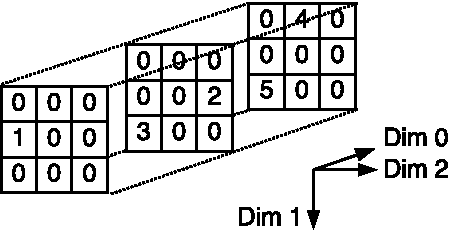
\includegraphics[width=2.5in]{images/tensorscooexpl.pdf} 
		\caption{A $3\times 3\times 3$ tensor}
        \label{fig:tensorCOO}
	\end{center}
\end{figure}
The tensor, illustrated in figure \ref{fig:tensorCOO}, of order $K = 3$ with shape $3\times 3 \times 3$ which has the following non-zero values :
\begin{center}
	\begin{tabular}{ l | c  }
		value & indexes\\ \hline
		1 & [0, 1, 0]\\ \hline
		2 & [1, 1, 2] \\ \hline
		3 & [1, 2, 0] \\ \hline
		4 & [2, 0, 1] \\ \hline
		5 & [2, 2, 0] \\ 
		
	\end{tabular}
\end{center}

It can be encoded with one values array and one indexes array :
\begin{figure}[h]
	\[
	\begin{aligned}
	Values_{(1\times NNZ)} = 
	\begin{bmatrix}
	1, &  2, & 3, & 4, & 5
	\end{bmatrix}
	\\
	Indexes_{(NNZ \times K)} = 
	\begin{bmatrix}
	[0, 1, 0] ,&  [1, 1, 2], & [1, 2, 0], & [2, 0, 1], & [2, 2, 0]
	\end{bmatrix}
	\end{aligned}
	\]
	\caption{A tensor stored in COO format}
		\label{fig:cooformattensor}
\end{figure}

